\documentclass[11pt, oneside]{article} 
\usepackage{geometry}
\geometry{letterpaper} 
\usepackage{graphicx}
	
\usepackage{amssymb}
\usepackage{amsmath}
\usepackage{parskip}
\usepackage{color}
\usepackage{hyperref}

\graphicspath{{/Users/telliott/Github/figures/}}
% \begin{center} \includegraphics [scale=0.4] {gauss3.png} \end{center}

\title{Irrational numbers}
\date{}

\begin{document}
\maketitle
\Large

There is a big problem with rational numbers which you probably know:  some numbers cannot be expressed as the ratio of two integers, as a first example, the number which when multiplied by itself is equal to $2$, written $\sqrt{2}$.  

The discovery that one cannot find integer $p$ and $q$ such that
\[ (\frac{p}{q})^2 = 2 \]
is due to the Pythagorean school and was most unwelcome since it screwed up their cherished theory of the universe.  

Some say that they drowned the guy who discovered it by throwing him overboard, and that his name was Hippasus.  Like most stories about Greek mathematicians, the truth is unknown.

We will see that there is a similar problem (called irrationality) with $\sqrt{3}$, $\sqrt{5}$, $\sqrt{7}$, etc., as well as with $3^{1/3}$ and so on.

Proof.

For $\sqrt{2}$:

We assume that there does exist a rational number $p/q$ such that
\[ \frac{p}{q} = \sqrt{2}  \]

We will show that this assumption leads to a contradiction.

A crucial part of the proof is that we suppose $p/q$ to be in lowest terms and in particular, that $p$ and $q$ are not both even.  It would be easy to recognize the case if they were both even, for then each would have their terminal digit in the set $\{ 0, 2, 4, 6, 8 \}$.

Another fact we will need is that every odd number, when squared, gives an odd result.  Proof:  every odd number can be written as $2k+1$ (for non-negative integer $k$) and then
\[ (2k+1)^2 = 4k^2 + 4k + 1 \]
which is an odd number.  Therefore, if $n^2$ is even, $n$ is also even.

So go back to 
\[ \frac{p}{q} = \sqrt{2}  \]

Move the $q$ term to the right-hand side and square both sides:
\[ p^2 = 2q^2 \]

This implies that $p^2$ and $p$ are even, using the result from above.   So we can write that $p = 2m$. But now
\[ (2m)^2 = 2q^2 \]
\[ 2m^2 = q^2 \]

which implies that $q$ is \emph{also} even.

We started with the assumption that $p$ and $q$ are not both even, but now we've reached a contradiction.  We conclude that there do not exist two integers $p$ and $q$ such that $p/q = \sqrt{2}$.

\subsection*{discussion}

To quote Hardy (\emph{A Mathematician's Apology}):

\begin{quote}
The proof is by reductio ad absurdum, and reductio ad absurdum, which Euclid loved so much, is one of a mathematician’s finest weapons. It is a far finer gambit than any chess gambit: a chess player may offer the sacrifice of a pawn or even a piece, but a mathematician offers \emph{the game}.
\end{quote}

The numbers like $\sqrt{2}$ are said to be \emph{irrational} numbers and the set of these, plus all the other numbers is called the set of real numbers $\mathbb{R}$.

This led Dedekind to formulate the famous Dedekind cut.  Visualize the standard number line as an infinite line on (an infinite) piece of paper.  

\begin{center} 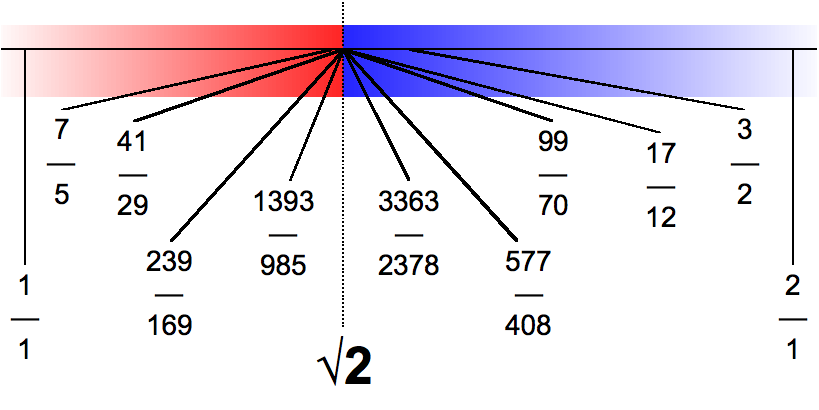
\includegraphics [scale=0.4] {Dedekind.png} \end{center}

Each real number corresponds to a cut, a knife-edge coming down somewhere on this number line.  Every other number that is not equal to this one, is either $>$ or $<$ the number specified by the cut.

One position is $\sqrt{2}$, another is $3/2$ and so on.

\subsection*{proof using prime factors}
The fundamental theorem of arithmetic says that any positive integer greater than $1$ can be expressed as a product of its prime factors
\[ n = p_1 \cdot p_2 \dots p_k \]
where this factorization is unique (if the factors are sorted first), and multiple copies allowed.  For example
\[ 60 = 2 \cdot 2 \cdot 3 \cdot 5 \]

A corollary says that the square of any integer (a perfect square) has an even number of prime factors since
\[ n^2 = p_1^2 \cdot p_2^2 \dots p_k^2 \]

In the expression from above
\[ p^2 = 2q^2 \]
the number of prime factors on the left is therefore even, but the number on the right is odd.  This is a contradiction.  Therefore $p$ and $q$ cannot both be integers.

\subsection*{continued fractions}
Square roots can be represented as continued fractions.  Some smart person figured out that we can write this:
\[ (\sqrt{2} - 1)(\sqrt{2} + 1) = 2 - 1 = 1 \]

Now, rearrange to get a substitution we will use repeatedly
\[ \sqrt{2} - 1 = \frac{1}{\sqrt{2} + 1} \]

Add one and subtract one on the bottom right:
\[ \sqrt{2} - 1 =  \frac{1}{2 + \sqrt{2} - 1} \]

And substitute for $\sqrt{2} - 1$:
\[ = \frac{1}{2 + \frac{1}{\sqrt{2} + 1}} \]

Lather, rinse, and repeat:
\[ = \frac{1}{2 + \frac{1}{2 + \sqrt{2} - 1}} = \frac{1}{2 + \frac{1}{2 + \frac{1}{\sqrt{2} + 1} }} \]

Clearly, this goes on forever.
\[ \sqrt{2} - 1 =  \cfrac{1}{2+\cfrac{1}{2+\cfrac{1}{2 + \dots}}}  \]

Add $1$ to the value of the \emph{continued fraction} to get an expression for the square root of $2$.

The numerators are all $1$, so this is called a simple continued fraction.  The continued fraction representation of $\sqrt{2}$ is usually written as $[1:2]$, meaning that there is an initial $1$ followed by repeated $2$'s.

This fraction goes on forever (since $\sqrt{2}$ is irrational).  One can view the existence of the infinite continued fraction as a proof of irrationality.

We can turn the above into an approximate decimal representation of $\sqrt{2}$, by truncating the infinite expansion at the $\dots$.  Then the last fraction is $5/2$.  Invert and add, repeatedly:

\begin{verbatim}
2 + 1/2 = 5/2
2 + 2/5 = 12/5
2 + 5/12 = 29/12
2 + 12/29 = 70/29
2 + 29/70 = 169/70
2 + 70/169 = 408/169
\end{verbatim}

To terminate we need to use that initial $1$:
\begin{verbatim}
1 + 169/408 = 577/408 = 1.414216
\end{verbatim}

To six places, $\sqrt{2} = 1.414213$.  We have five places, and can easily get more.

\subsection*{geometric proof}

There are many other proofs of the irrationality of the square root of $2$.

\url{https://www.cut-the-knot.org/proofs/sq_root.shtml}

Here we will look at one more, before considering a more general proof for all non-perfect squares.  This one is from Tom Apostol (see the link).  A more elaborate exposition is:

\url{https://jeremykun.com/2011/08/14/the-square-root-of-2-is-irrational-geometric-proof/}

Draw an isosceles triangle with side length $1$, then Pythagoras tells us that the hypotenuse is equal in length to $\sqrt{2}$ (left panel).

Our hypothesis is that this length is a rational number, and its ratio to the side is in "lowest terms".

\begin{center} 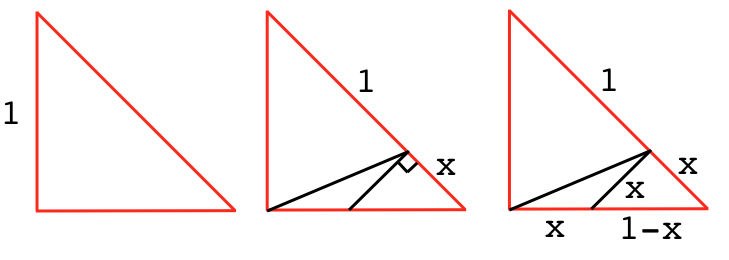
\includegraphics [scale=0.4] {sqrt2e.png} \end{center}

Mark off the length of the side (length $1$) on the hypotenuse, and erect a perpendicular (middle panel).  Also draw the line segment to the opposite vertex of the original triangle.

The new small triangle that is formed containing the right angle and with side length $x$ in the middle panel is isosceles, because it is a right triangle, and it  contains one of the complementary angles of the original right triangle.

By hypothesis, its side length $x$ is the difference of two rational numbers, so $x$ is a rational number.

Furthermore, the \emph{other} small triangle is also isosceles.  Its base angles, when added to the equal angles of an isosceles triangle, form right angles.  This allows us to mark the side along the base as having length $x$ as well.

Therefore, the hypotenuse of the new, small right triangle is a rational number, since it is equal to $1 - x$.

We are back where we started, with an isosceles triangle that has all rational sides.  

It is clear that this process can continue forever.  The sides will never be in "lowest terms" because we can always form a new similar but smaller right triangle, which amounts to evenly dividing both the sides and the hypotenuse by a rational number.

\subsection*{general proof}

I found a long algebraic proof of the general irrationality of roots and I wrote it up the big calculus book.  But then I came upon simple elegant proof based on the fundamental theorem of arithmetic.

We suppose that there exist two integers $a$ and $b$ such that 
\[ (\frac{a}{b})^2 = n \]

Both $a$ and $b$ have a unique prime factorization.  Suppose that gives $a = a_1 \cdot a_2 \dots a_i$ and likewise for $b$ so:
\[ (\frac{a_1 \cdot a_2 \dots a_i}{b_1 \cdot b_2 \dots b_j})^2 = n \]

There must be at least some $b_j$ which are not $a_i$, otherwise we could cancel all of them and so $a/b$ would be an integer.

Call that factor or factors $q$, so in lowest terms we have
\[ (\frac{a_1 \cdot a_2 \dots }{q_1 \dots q_k})^2 = n \]

But then, after squaring, we will have $q_1^2$ (for example) in the denominator and no corresponding factor of either $q_1$ or $q_1^2$ in the numerator.  

The $q_k$ cannot be canceled and so the result cannot be an integer.

This proves that the only $n$ with rational square roots are perfect squares with integer roots.

The proof also applies generally to other powers like cube and the fourth and fifth power and so on.

\subsection*{other irrational numbers}

There are many other irrational numbers besides these square roots.  

The proof that $e$ is irrational is easy, but since we haven't introduced the exponential yet we need to wait.  The proof that $\pi$ is irrational is bit harder, we will skip that.

\section*{density}

\subsection*{number line}
A simple tool to visualize all of the real numbers is the familiar number line.  Here is the number line with numbers marked from $\mathbb{N}$, but obviously we could also draw one for $\mathbb{Z}$ or $\mathbb{Q}$.

We explore the application of the number line to $\mathbb{R}$ as we proceed.
\begin{center} 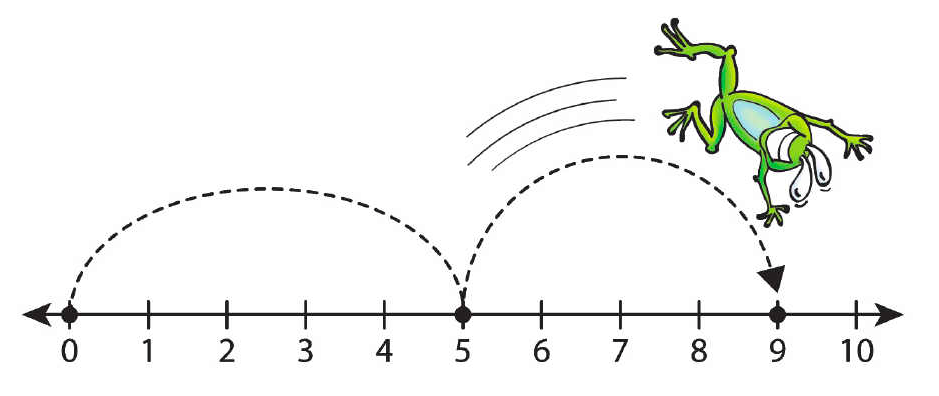
\includegraphics [scale=0.4] {number_line.png} \end{center}

We might simply assume that to every point on the number line there corresponds a rational or irrational number, and that this total collection obeys the same laws of arithmetic as the rational numbers do.

As mentioned above, the need for the real numbers is indicated by empty "holes" in the number line corresponding to the irrational numbers like $\sqrt{2}$.

A problem that arises is how to specify an irrational number non-geometrically and other than as the solution to an equation such as $r^2 = 2$.  We saw above a method involving continued fractions.

\subsection*{approximations}

In all cases we write particular real numbers as \emph{approximations}.  For example, the square root of $2$ lies between $1$ and $2$ because
\[ 1^2 = 1 < 2 \]
\[ 2^2 = 4 > 2 \]

Implying that $\sqrt{2} < 2$.  At the second place:
\[ 1.4^2 = 1.96 < 2 \] 
\[1.5^2 = 2.25 > 2 \]

Implying that $\sqrt{2} < 1.5$.  At the third:
\[ 1.41^2 = 1.9881 < 2 \]
\[1.42^2 = 2.0164 > 2 \]

Implying that $\sqrt{2} < 1.42$.  

This process may be continued for as long as desired.

We can never write down the decimal value of $\sqrt{2}$ exactly, but only approximate it to greater and greater precision.  It goes on forever.

In carrying out this recursive process, suppose we know $1.41$ and we seek the next digit.  One way is to just try all the digits in order starting with $1$.

\url{https://gist.github.com/telliott99/79178d6752b6f7b9325476a64bc82953}

In this Python code, I have dispensed with the decimal point to make the math easier.  We generate a sequence of integers starting with 

\begin{verbatim}
14
141
1414
14142
..
\end{verbatim}

This code generates 1000 digits of the value instantly.

However, rather than try all the digits in order starting with $1$, there is a better way, which is to try to estimate the error

For example $141^2 = 19881$ so we are short of $20000$ by $119$.  

$142^2 = 20164$ so the difference is $283$ and the fraction of the difference that we're under is $119/283 = 0.4205$.  In fact, the next two digits of the approximation to $\sqrt{2}$ are $42$.

Rather than implement this idea, we will see a better method for obtaining the value in calculus, called the Newton or Newton-Raphson method.

At the seventh place
\[ 1.414213^2 = 1.9999984093689998.. < 2 \]
\[ 1.414214^2 = 2.0000012377960004 > 2 \]

Because any repeating decimal can be written as a fraction, we know that the sequence cannot repeat (any apparent repeat will be illusory).  

It is a curious fact that all the digits of $\pi$, \emph{to whatever accuracy you desire}, can be found in the correct order, somewhere within the digital expansion of $e$ or $\phi$ or indeed, any irrational number.  The converse is also true.

Another way to say the same thing is that \emph{any} finite sequence can be found within \emph{any} infinite sequence, and in as many copies as you have the patience to discover.  The sequence 271828 is found starting around digit 33,790 of $\pi$, but 2718281 (adding the next digit of $e$) is not found within the first million digits of $\pi$.  You just need more.

\subsection*{limit of a sequence}

The real number $\sqrt{2}$ is defined to be the limit of the sequence 

$1.4, 1.41, 1.414, \dots 1.414214 \dots$ 

as the number of terms $n \rightarrow \infty$.

In a similar way, the number $e$ can be viewed as
\[ \lim_{n \rightarrow \infty} (1 + \frac{1}{n})^n \]

And the number $\pi$ can be viewed as the limit of the method of exhaustion applied to the area of a unit circle.

\subsection*{density of numbers}

We showed previously that between any two rational numbers, including $0$ and the \emph{smallest} positive number, one can find another rational number which lies between them.

Three related statements are also true.

$\bullet$ for any two rational numbers one can find a real number which lies between them

$\bullet$ for any two real numbers one can find a rational number which lies between them

$\bullet$ for any two real numbers one can find a real number which lies between them

Proofs of these are readily accessible but we'll do only one, for the sake of brevity.

\subsection*{theorem}

$\bullet$  Between any two rational numbers it is always possible to find a real number.

Proof.

We will find a \emph{particular} irrational in the interval $(a,b)$, where $a$ and $b$ are rational.  For $a < b$, we simply add to the number $a$ the following
\[ c = \frac{b - a}{\sqrt{2}} = \frac{\sqrt{2}}{2}(b - a) \]

$c$ is smaller than $b - a$ (because $\sqrt{2}/2 < 1$) so the result $a + c$ lies between $a$ and $b$.  

We also know that $c$ is irrational, because $\sqrt{2}$ times any rational number is irrational.  Finally, $a + c$ is irrational because adding $\sqrt{2}$ times a rational number to any rational number produces an irrational number.

Proof of the first preliminary requirement:  $\sqrt{2}$ times a rational is irrational.  Suppose for integer $p, q, r, s$ we have
\[ \sqrt{2} \ \frac{p}{q} = \frac{r}{s} \]
then
\[ \sqrt{2} = \frac{rq}{ps} \]
But the right-hand side is rational, so this is a contradiction.

For the second requirement, again by contradiction suppose
\[ \sqrt{2} \ \frac{p}{q} +  \frac{s}{t} = \frac{u}{v} \]
for integer $p, q, r, s, u, v$.  But the right-hand side of
\[ \sqrt{2} = \frac{q}{p} ( \frac{u}{v} - \frac{s}{t}) \]
is rational, so this is a contradiction.

$\square$

Note in passing that powers are different.  What do you think about
\[ r = \sqrt{2}^{\sqrt{2}} \]
You may think $r$ is "likely" to be irrational.  Just a mess.  But how about
\[ r^{\sqrt{2}} \]
Whether $r$ is rational or irrational
\[ r^{\sqrt{2}} = (\sqrt{2}^{\sqrt{2}})^{\sqrt{2}} = \sqrt{2}^2 = 2 \]


This property of the real (and even the rational) numbers, that there is no closest number to any given number, accounts for virtually all of the theoretical difficulties in calculus which are solved by the use of limits and the apparatus of $\delta$ and $\epsilon$ or alternatively, neighborhoods.  We will get to that in a bit.

\end{document}